\newpage
\appendix
\section{Anhang}\label{sec:anhang}

\subsection{Unsicherheiten}\label{sec:unsicherheiten}

Alle Unsicherheiten werden nach dem GUM bestimmt und berechnet.
Die Gleichungen dazu finden sich in \ref{fig:GUM_combine} und \ref{fig:GUM_formula}.
Hierfür wurde die Python Bibliothek "uncertainties" verwendet, welche den Richtlinien des GUM folgt.
Für die Unsicherheiten der Parameter in Annäherungskurven wurden die $y$-Unsicherheiten der anzunähernden Werte beachtet und die Methode der kleinsten Quadrate angewandt.
Dafür steht in der Bibliothek die Methode "scipy.optimize.curve\_fit()" zur Verfügung.

Für digitale Messungen wird eine rechteckige Verteilung mit $\sigma_X = \frac{\Delta X}{2\sqrt{3}}$ und für analoges Ablesen wird eine Dreiecksverteilung mit $\sigma_X = \frac{\Delta X}{2\sqrt{6}}$ angenommen.
Die jeweiligen $\Delta X$ sind im entsprechenden Abschnitt zu finden.

\begin{figure}[ht]
	\begin{equation*}
	x = \sum_{i=1}^{N} x_i
	;\quad
	\sigma_x = \sqrt{\sum_{i = 1}^{N} \sigma_{x_i}^2}
	\end{equation*}
	\caption{Formel für kombinierte Unsicherheiten des selben Typs nach GUM.}
	\label{fig:GUM_combine}
\end{figure}

\begin{figure}[ht]
	\begin{align*}
	f = f(x_1, \dots , x_N)
	;\quad
	\sigma_f = \sqrt{\sum_{i = 1}^{N}\left(\pdv{f}{x_i} \sigma_{x_i}\right) ^2}
	\end{align*}
	\caption{Formel für sich fortpflanzende Unsicherheiten erster Ordnung nach GUM.}
	\label{fig:GUM_formula}
\end{figure}

\newpage
\subsection{weitere Abbildungen}

\begin{figure}[H]
	\centering
	\begin{subfigure}[c]{.45\textwidth}
		\centering
		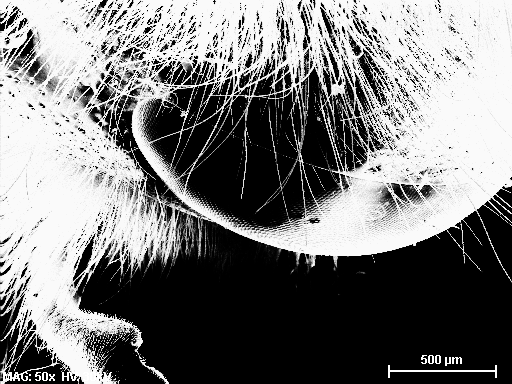
\includegraphics[width=.8\textwidth]{raw/SEM/Hummelauge_M0050}
		\subcaption{x50}
	\end{subfigure}
	\begin{subfigure}[c]{.45\textwidth}
		\centering
		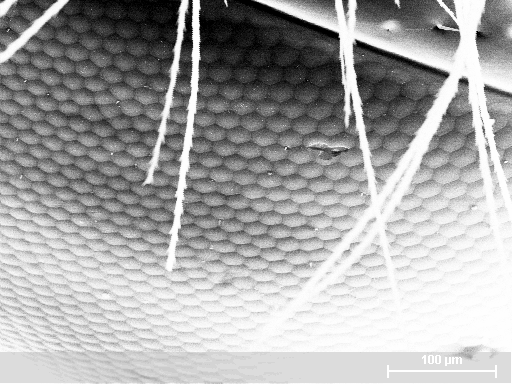
\includegraphics[width=.8\textwidth]{raw/SEM/Hummelauge_M0252}
		\subcaption{x252}
	\end{subfigure}
	\begin{subfigure}[c]{.45\textwidth}
		\centering
		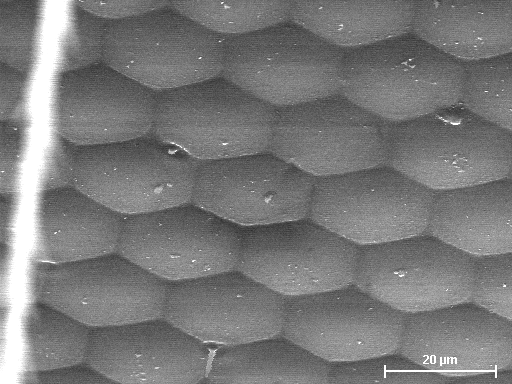
\includegraphics[width=.8\textwidth]{raw/SEM/Hummelauge_M1300}
		\subcaption{x1300}
	\end{subfigure}
	\begin{subfigure}[c]{.45\textwidth}
		\centering
		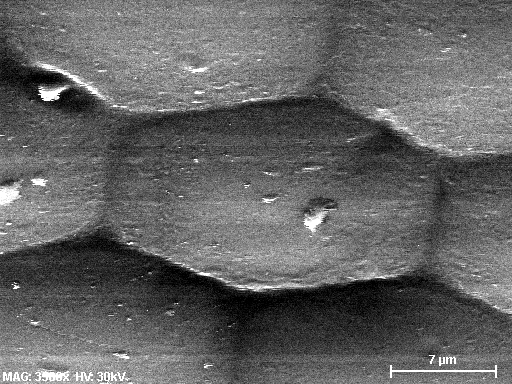
\includegraphics[width=.8\textwidth]{raw/SEM/Hummelauge_M3500}
		\subcaption{x3500}
	\end{subfigure}
	\begin{subfigure}[c]{.45\textwidth}
		\centering
		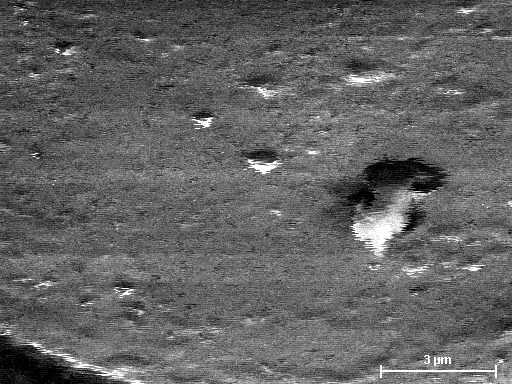
\includegraphics[width=.8\textwidth]{raw/SEM/Hummelauge_M9010}
		\subcaption{x9010}
	\end{subfigure}
	\caption{SEM-Bild eines Hummelauges bei unterschiedlichen Vergrößerungen.}
	\label{fig:Hummelauge}
\end{figure}

\begin{figure}[H]
	\centering
	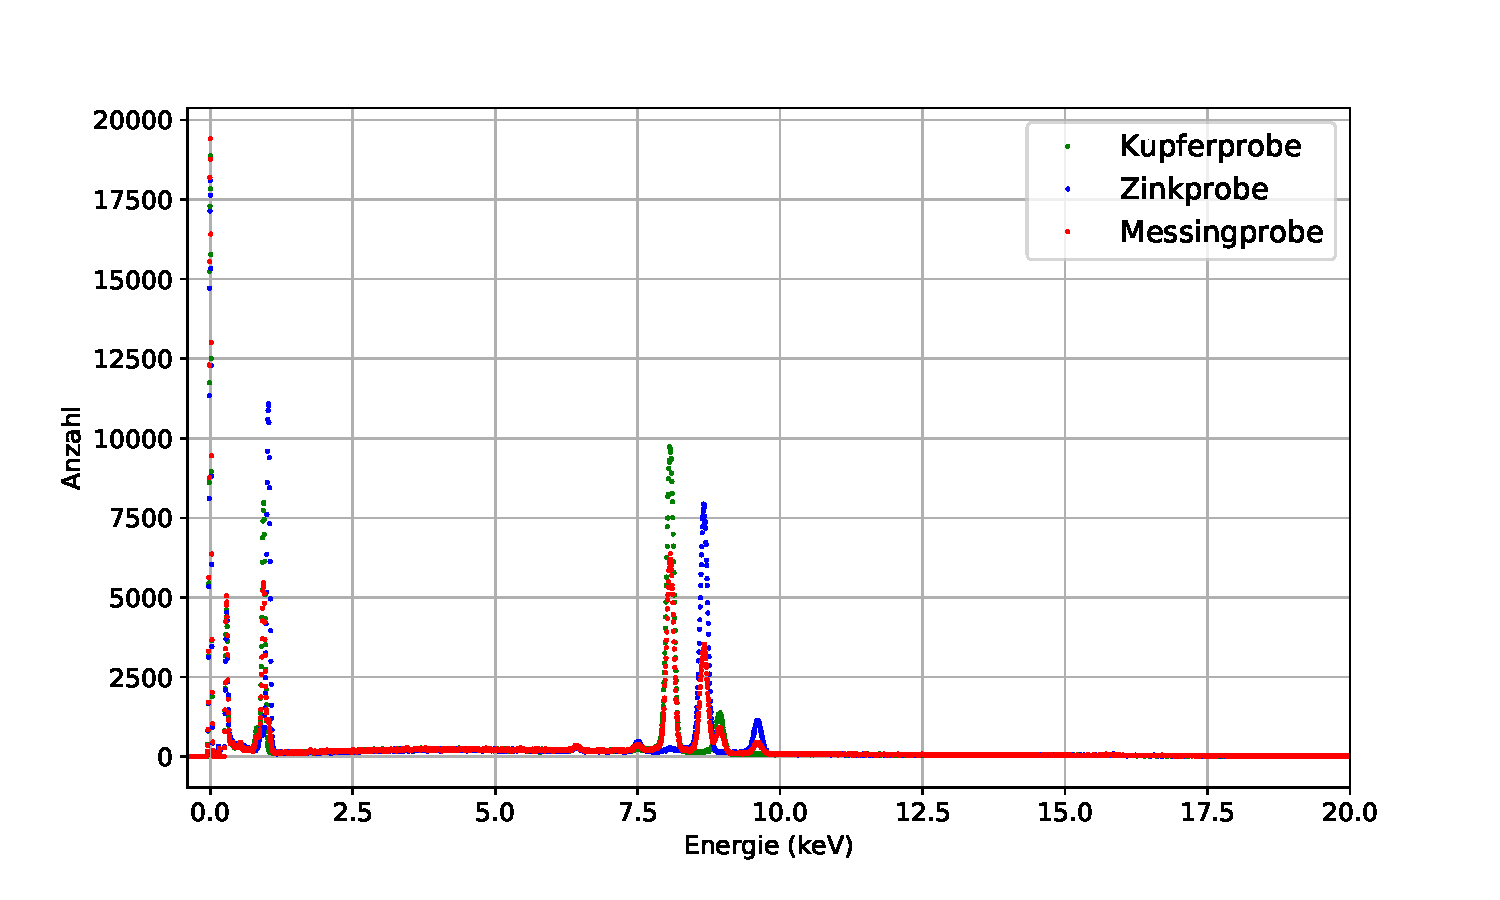
\includegraphics[width=.8\textwidth]{plots/KupferprobeGanz}
	\caption{Röntgen-Absorptionsspektrum von Kupfer und Zink für eine Messing-, Kupfer- und Zinkprobe.}
	\label{fig:messing_spektrum}
\end{figure}

\begin{figure}[H]
	\centering
	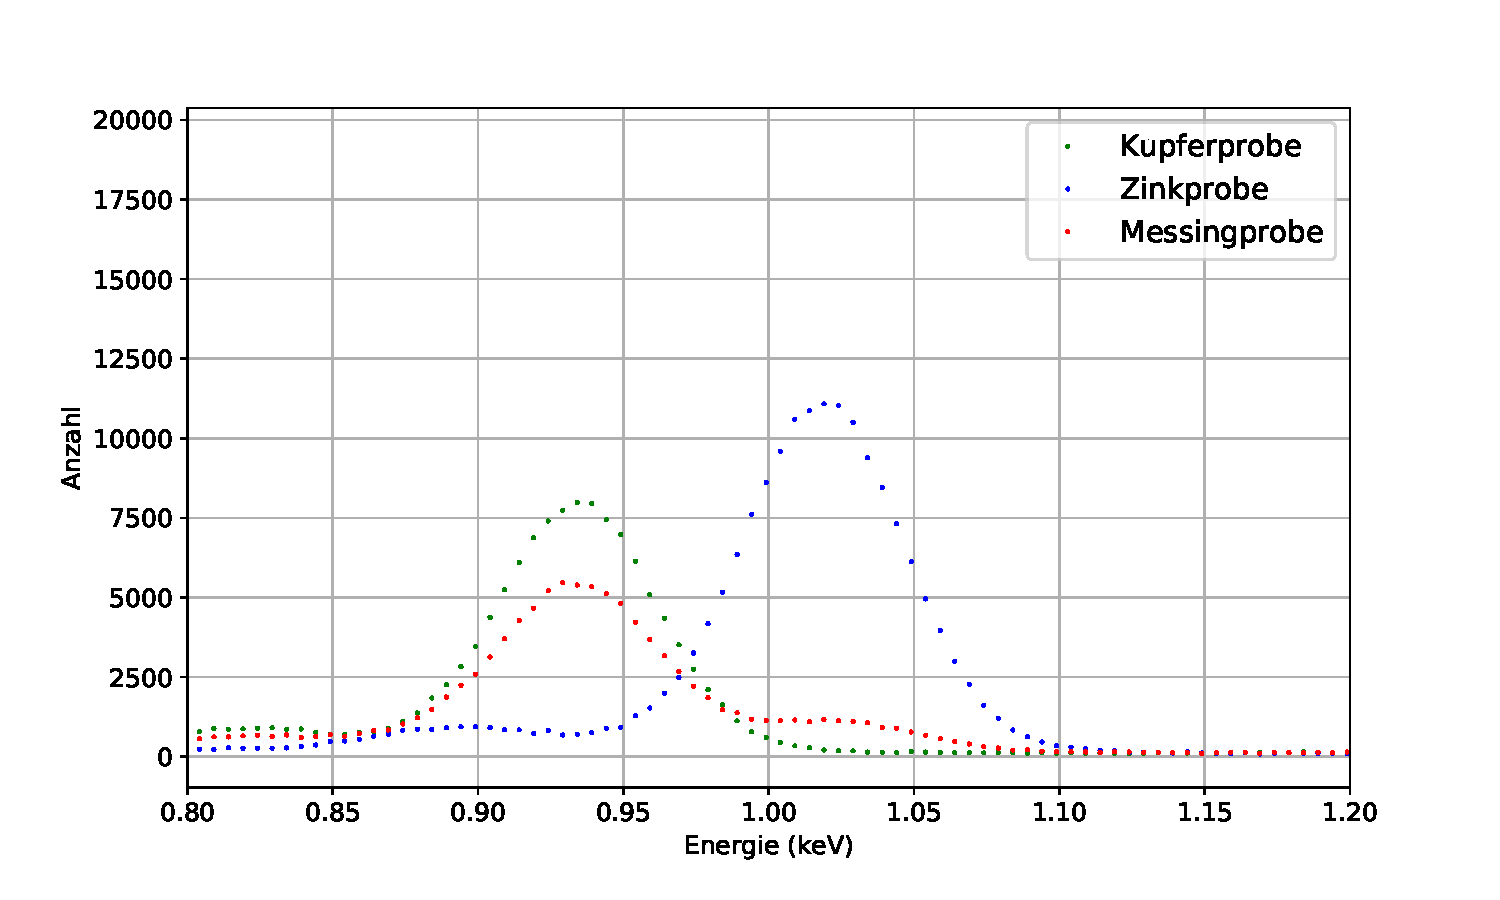
\includegraphics[width=.8\textwidth]{plots/KupferprobeL}
	\caption{Röntgen-Absorptionsspektrum im Bereich der $L$-Linien von Kupfer und Zink für eine Messing-, Kupfer- und Zinkprobe. Zwischen $L_\alpha$ und $L_\beta$ kann nicht unterschieden werden.}
	\label{fig:l-linien}
\end{figure}
